% ----- Consignes exo 31 ----- %
\begin{td-exo}[Le problème du stable dans un graphe]\,\\ % 31 
	On rappelle la définition suivante:
	\begin{definition}
		Un \defemph{stable} dans un graphe est un ensemble de sommets qui sont deux à deux non adjacents.
	\end{definition}
	La matrice d'incidence (arêtes-sommets) \(A = (a_{ij})\) est une matrice \(m \times n\) définie de la manière suivante:
	\begin{equation*}
		a_{ij} = \begin{cases}
			1 & \text{si l'arête } i \text{ est incidente au sommet } j,\\
			0 & \text{sinon.}
		\end{cases}
	\end{equation*}

	\begin{enumerate}
		\item Donner la matrice d'incidence du graphe donné par la figure~\ref{fig:td4_ex31_f1}:

		\ffigbox[\FBwidth]{%
\caption{\centering Un graphe non orienté}\label{fig:td4_ex31_f1}
}{
    \fbox{
        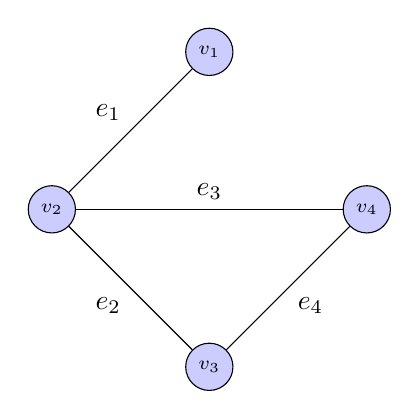
\begin{tikzpicture}[scale=1, main node/.style={circle, draw, fill=blue!20, inner sep=1pt, font=\scriptsize, minimum size=6mm, text=black}]
            % les sommets initiaux
            \node[main node] (v1) at (0,0) {\(v_1\)};
            \node[main node] (v2) at (-2,-2) {\(v_2\)};
            \node[main node] (v3) at (0,-4) {\(v_3\)};
            \node[main node] (v4) at (2,-2) {\(v_4\)};

            % les arcs avec capacités
            \draw (v1) to node[above left] {\(e_1\)} (v2);
            \draw (v2) to node[below left] {\(e_2\)} (v3);
            \draw (v2) to node[above] {\(e_3\)} (v4);
            \draw (v3) to node[below right] {\(e_4\)} (v4);

        \end{tikzpicture}
    }
}

		\item Le problème de trouver un stable maximum dans un graphe ci-dessus peut se formuler comme un programme linéaire.
		Donner cette formulation.
	\end{enumerate}
\end{td-exo}

% ----- Solutions exo 31 ----- %
\iftoggle{showsolutions}{ 
	\begin{td-sol}[]\ % 31
		
	\end{td-sol}
}{}
